%%%%%%%%%%%%%%%%%%%%%%%%%%%%%%%%%%%%%%%
% Wenneker Resume/CV
% LaTeX Template
% Version 1.1 (19/6/2016)
%
% This template has been downloaded from:
% http://www.LaTeXTemplates.com
%
% Original author:
% Frits Wenneker (http://www.howtotex.com) with extensive modifications by
% Vel (vel@LaTeXTemplates.com)
%
% License:
% CC BY-NC-SA 3.0 (http://creativecommons.org/licenses/by-nc-sa/3.0/
%
%%%%%%%%%%%%%%%%%%%%%%%%%%%%%%%%%%%%%%

%----------------------------------------------------------------------------------------
%	PACKAGES AND OTHER DOCUMENT CONFIGURATIONS
%----------------------------------------------------------------------------------------

\documentclass[a4paper,12pt]{memoir} % Font and paper size

%%%%%%%%%%%%%%%%%%%%%%%%%%%%%%%%%%%%%%%%%
% Wenneker Resume/CV
% Structure Specification File
% Version 1.1 (19/6/2016)
%
% This file has been downloaded from:
% http://www.LaTeXTemplates.com
%
% Original author:
% Frits Wenneker (http://www.howtotex.com) with extensive modifications by 
% Vel (vel@latextemplates.com)
%
% License:
% CC BY-NC-SA 3.0 (http://creativecommons.org/licenses/by-nc-sa/3.0/)
%
%%%%%%%%%%%%%%%%%%%%%%%%%%%%%%%%%%%%%%%%%

%----------------------------------------------------------------------------------------
%	PACKAGES AND OTHER DOCUMENT CONFIGURATIONS
%----------------------------------------------------------------------------------------

\usepackage{XCharter} % Use the Bitstream Charter font
\usepackage[utf8]{inputenc} % Required for inputting international characters
\usepackage[T1]{fontenc} % Output font encoding for international characters

\usepackage[top=1cm,left=1cm,right=1cm,bottom=1cm]{geometry} % Modify margins

\usepackage{graphicx} % Required for figures

\usepackage{flowfram} % Required for the multi-column layout

\usepackage{url} % URLs

\usepackage[usenames,dvipsnames]{xcolor} % Required for custom colours

\usepackage{tikz} % Required for the horizontal rule

\usepackage{enumitem} % Required for modifying lists
\setlist{noitemsep,nolistsep} % Remove spacing within and around lists

\setlength{\columnsep}{\baselineskip} % Set the spacing between columns

% Define the left frame (sidebar)
\newflowframe{0.2\textwidth}{\textheight}{0pt}{0pt}[left]
\newlength{\LeftMainSep}
\setlength{\LeftMainSep}{0.2\textwidth}
\addtolength{\LeftMainSep}{1\columnsep}
 
% Small static frame for the vertical line
\newstaticframe{1.5pt}{\textheight}{\LeftMainSep}{0pt}
 
% Content of the static frame with the vertical line
\begin{staticcontents}{1}
\hfill
$%\tikz{\draw[loosely dotted,color=RoyalBlue,line width=1.5pt,yshift=0](0,0) -- (0,\textheight);}
\hfill\mbox{}
\end{staticcontents}
 
% Define the right frame (main body)
\addtolength{\LeftMainSep}{1.5pt}
\addtolength{\LeftMainSep}{1\columnsep}
\newflowframe{0.7\textwidth}{\textheight}{\LeftMainSep}{0pt}[main01]

\pagestyle{empty} % Disable all page numbering

\setlength{\parindent}{0pt} % Stop paragraph indentation

%----------------------------------------------------------------------------------------
%	NEW COMMANDS
%----------------------------------------------------------------------------------------

\newcommand{\userinformation}[1]{\renewcommand{\userinformation}{#1}} % Define a new command for the CV user's information that goes into the left column

\newcommand{\cvheading}[1]{{\Huge\bfseries\color{RoyalBlue} #1} \par\vspace{.6\baselineskip}} % New command for the CV heading
\newcommand{\cvsubheading}[1]{{\Large\bfseries #1} \bigbreak} % New command for the CV subheading

\newcommand{\Sep}{\vspace{1em}} % New command for the spacing between headings
\newcommand{\SmallSep}{\vspace{0.5em}} % New command for the spacing within headings

\newcommand{\aboutme}[2]{ % New command for the about me section
\textbf{\color{RoyalBlue} #1}~~#2\par\Sep
}
	
\newcommand{\CVSection}[1]{ % New command for the headings within sections
{\Large\textbf{#1}}\par
\SmallSep % Used for spacing
}

\newcommand{\CVItem}[2]{ % New command for the item descriptions
\textbf{\color{RoyalBlue} #1}\par
#2
\SmallSep % Used for spacing
}

\newcommand{\bluebullet}{\textcolor{RoyalBlue}{$\circ$}~~} % New command for the blue bullets
 % Include the file specifying document layout and packages

%----------------------------------------------------------------------------------------
%	NAME AND CONTACT INFORMATION
%----------------------------------------------------------------------------------------

\userinformation{ % Set the content that goes into the sidebar of each page
\begin{flushright}
% Comment out this figure block if you don't want a photo
% 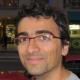
\includegraphics[width=0.6\columnwidth]{photo.jpg}\\[\baselineskip] % Your photo
\small % Smaller font size
Álvaro González \\ % Your name
\url{alvaroga@gmail.com} \\ % Your email address
+41 754 118 512 \\ % Your phone number
\Sep % Some whitespace
\textbf{Address} \\
Avenue D'Aïre 93F \\ % Address 1
Geneve, 1203 \\ % Address 2
\textbf{Nationality} \\
	Spanish 
\includegraphics{spain.png}\\ % Nationality
\vfill % Whitespace under this block to push it up under the photo
\end{flushright}
}

%----------------------------------------------------------------------------------------

\begin{document}

\userinformation % Print your information in the left column

\framebreak % End of the first column

%----------------------------------------------------------------------------------------
%	HEADING
%----------------------------------------------------------------------------------------

\cvheading{Álvaro González Álvarez} % Large heading - your name

\cvsubheading{Service Manager} % Subheading - your occupation/specialization

%----------------------------------------------------------------------------------------
%	ABOUT ME
%----------------------------------------------------------------------------------------

\aboutme{About Me}{Service manager in the IT-CDA-WF section, working to offer services to CERN's developer community. In a continuous effort to improve and expand the current services and the technologies that make them possible. User oriented person.}
%----------------------------------------------------------------------------------------
%	COMPETENCES
%----------------------------------------------------------------------------------------

\CVSection{Competences} % From the competency model

{\begin{tabular}{p{0.23\textwidth} p{0.23\textwidth} p{0.23\textwidth}}
\bluebullet Managing self & \bluebullet Achieving results & \bluebullet Learning and Sharing Knowledge\\
\bluebullet Solution architecture &  \bluebullet Systems integration & \bluebullet Configuration management\\
\bluebullet Application support &  \bluebullet Problem management & \bluebullet Availability management\\
\end{tabular}}

\CVSection{Experience}

%------------------------------------------------

\CVItem{October 2008 - present, \textit{PJAS, Fellow, and Staff}, CERN}{

\:
\:

\begin{itemize}
    \item [Since 2015] Part of the GitLab (GiT) team. In its two years of life GitLab has risen to host ~20000 projects and ~10000 users, including services like CI (Continuous Integration) and a Docker registry. It uses container orchestration technologies like Openshift and Docker. Tasks include user support and upgrade operations. Based in Ruby and Openshift.
    \item [Since 2015] CERNforge portal developing and operations. Since 2012, users can create, administrate and delete developing resources. Focusing now in JIRA's features. Based in Django and Openshift.
    \item [Since 2014] Secretary in monthly AMS-COMPASS-NA62-WA105 coordination meeting. Tasks include minutes compilation, consultancy, and coordination between experiments and IT experts.
    \item [Since 2012] Gitolite (GiT) service manager. Closed in favour of GitLab in July 2017. The service served as an alternative to Subversion when GitLab was not yet ready for production. Based in Puppet VMs and a Perl access control system.
    \item [Since 2012] JIRA service manager. Currently hosting ~1000 projects and serving ~49000 users. The service offers two instances to a general CERN audience and two private instances to SFT and Alice respectively. Plugins have been developed in Java to integrate JIRA with the CERN infrastructure (mainly SSO and eGroups). Tasks include plugin development, operations, and user support and consultancy.
    \item [Since 2009] Subversion service manager. The service is planned for closure during LS2, this means no new projects or service development. The current focus is to help users to migrate to GitLab. It still holds ~2400 projects and ~1700 people use it. This includes several key projects. For example Atlas , Accelerator controls, and CMS have active projects. Applications like Trac and WebSVN are provided as web interfaces.
    \item [Since 2008] Linux engineering license servers. This includes licenses for Mathematica, MATLAB, Intel, Cadence, and more. These software products are used by hundreds of people to perform key engineering tasks at CERN. Tasks include license installation and problem resolution.
\end{itemize}}

\clearpage % Start a new page
\userinformation % Print your information in the left column
\framebreak % End of the first columN

\CVItem{November 2007 - September 2008, \textit{IT specialist}, Herca}{
Small construction company, developing a "Smart Hotel".
\begin{itemize}
	\item Skill learned: Problem solving with no help and limited resources.
	\item Responsibilities: All computer related tasks, including purchases, installation, software developing.
\end{itemize}
}

%------------------------------------------------

\Sep % Extra white space after the end of a major section


%----------------------------------------------------------------------------------------
%	Education
%----------------------------------------------------------------------------------------

\CVSection{Education}

\CVItem{University}{
\begin{itemize}
	\item October 2000 - September 2004, \textit{Universidad de Oviedo, Spain}. Bachelor.
	\item August 2005 - December 2005, \textit{University of North Carolina, USA}
	\item October 2004 - September 2007, \textit{Universidad de Oviedo, Spain}. Master.
\end{itemize}
}

\CVItem{Languages}

{\begin{tabular}{p{0.3\textwidth} p{0.4\textwidth}}
	\bluebullet Spanish, Native &  \bluebullet English, Fluent (C1) \\
	\bluebullet French, Intermediate (B1) \\
\end{tabular}}

\CVItem{Trainings}{
\begin{itemize}
        \item 2009-2010, General and Professional French courses
	\item 2009, Developing secure software
	\item 2009, Secure coding for Perl
	\item 2011, Communicating to Convince
	\item 2014, Making presentations
	\item 2015, Object-oriented Design Patterns
        \item 2015, Personal Awareness \& Impact
        \item 2016, Balancing Performance and Pressure
\end{itemize}
}

\CVItem{Conferences}{
\begin{itemize}
    \item HEPIX 2011, Darmstadt, Germany.
    \item CHEP 2012, New York, USA.
    \item HEPIX 2013, Bologna, Italy.
    \item HEPIX 2014, Annecy, France.
\end{itemize}}
%------------------------------------------------

\Sep

\end{document}
